\begin{frame}{PyGame Breakout}
	\begin{block}{}
	Starting from the work presented in \cite{DBLP:journals/corr/abs-1807-06333} the agents were trained on a modified PyGame Breakout with a $6\times18$ grid.
	\end{block}
	
	\begin{block}{}
	Game state already stored inside the class instance (ball position, paddle position, blocks status).
	\end{block}
	
\end{frame}

\begin{frame}{Atari Breakout}
    \begin{columns}[c,onlytextwidth]
        \column{0.65\textwidth}
	        \begin{block}{}
            Breakout from OpenAI Gym: toolkit for comparing learning algorithm. Provides easy access to state and reward. No assumption on the agent.
            \end{block}
        
	        \begin{block}{}
	        	Class stores pixels status. Need to extract information about the game state from it.
	        \end{block}

            \begin{block}{}
	            The environment is more stochastic.
			\end{block}
		
        \column{0.3\textwidth}
            \begin{figure}
                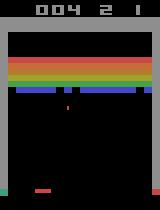
\includegraphics[width=\textwidth]{images/gym-breakout-image-example.jpg}
            \end{figure}
    \end{columns}
\end{frame}
